% Copyright (c) 2014,2016 Casper Ti. Vector
% Public domain.

\chapter{预备知识介绍}
\section{HBase简介}
HBase是Hadoop 生态系统中一个列式NoSQL数据库,基于BigTable\supercite{bigtable}模型设计,搭建在HDFS(Hadoop分布式文件系统)之上。

\begin{figure}[htbp]
\centering
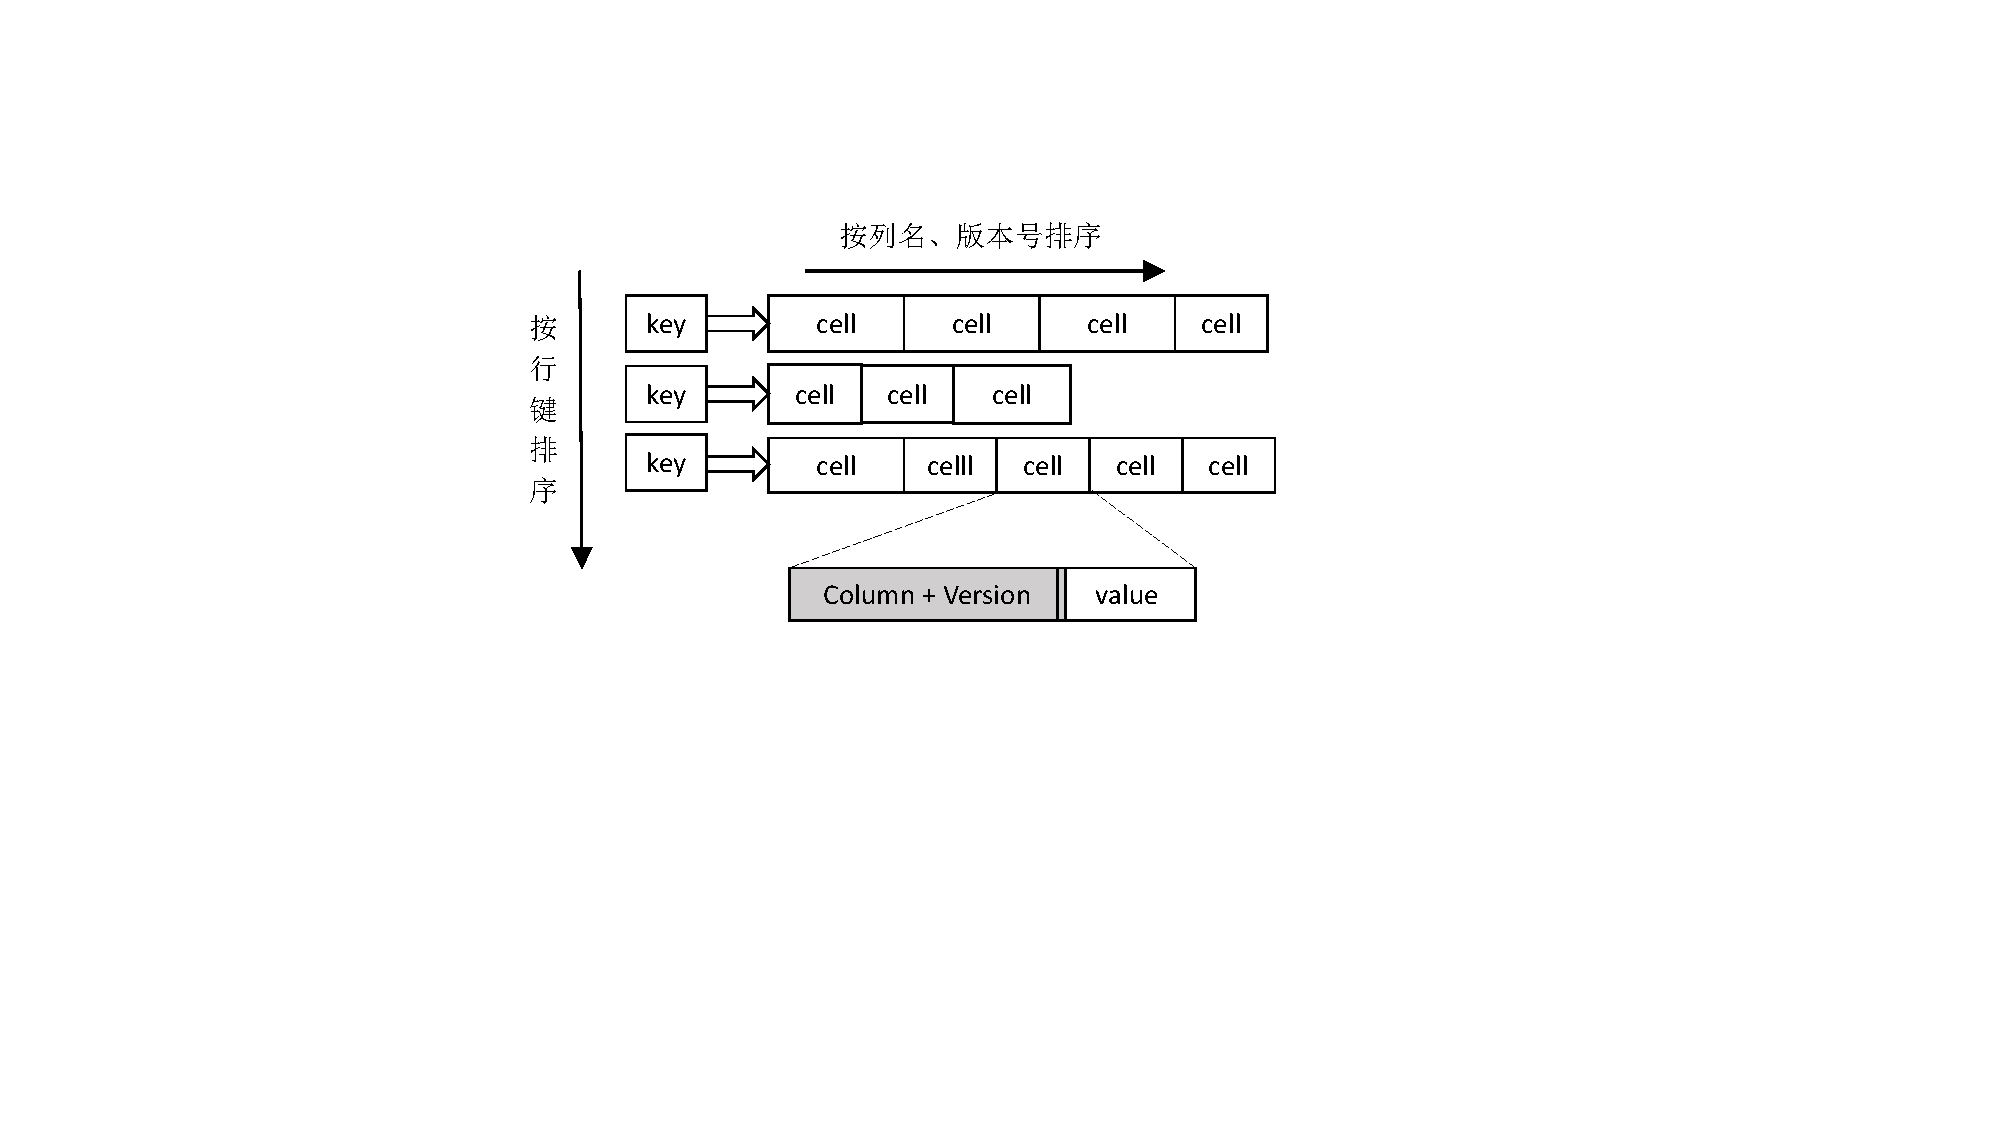
\includegraphics[width=100mm]{fig/big_table.pdf}
\caption{BigTable模型示例}
\label{fig:big_table}
\end{figure}

BigTable是Google在2008年提出的一个处理海量数据的NoSQL数据库。图\ref{fig:big_table}是BigTable的模型示例。在BigTable的模型中,数据表以行为单位组织,每行由一个键值唯一标识,称为行键(rowkey)。一行中可以包含任意数目的单元格(cell),每个单元格由列名、版本号(时间戳)和值(value)组成。BigTable中的行是以行键排序的,每一行中的单元格又是以列名和版本号进行排序,这使得其与关系数据库一样能快速定位到目标单元格。区别于传统关系模型,BigTable中的列名不需要事先定义,因为其底层实际为一个Key-Value 存储,就如数据结构Map不需要事先定义所有key。每个列名从属于一个列族,只有列族需要在定义表结构时给出。
HBase提供对某一行数据的Put、Get、Delete接口,能够具体操作该行中的给定列。另外,HBase提供给定行键范围的Scan接口,可以快速地获得连续几行的数据。Scan接口也可指定特定的列或附加Filter来过滤无关数据。
HBase由于其优异的可扩展性和稳定性,在产业界得到了广泛应用。

\section{图数据库Titan}
图数据库是以图的形式来表示和管理数据的数据库\supercite{graph_models_survey},与传统的关系型数据库相比,图数据库在图结构相关的查询上有更优异的性能,如多跳邻域查询、路径查询、局部聚集系数计算等。
Titan是一个基于Blueprints 接口设计的开源图数据库,其实现了一个可插拔的存储接口,可以部署在BerkerlyDB 、HBase或Cassandra\supercite{cassandra}之上。相比于著名的图数据库Neo4j\supercite{neo4j},Titan是完全开源免费的,其受关注度正在与日俱增。而且由于Hadoop生态系统在产业界的广泛应用,在HBase上搭建Titan,即使用Titan on HBase应对图处理需求是较为常见的选择。
在图数据库Titan中,基于BigTable模型,数据在HBase中以邻接表的形式存储,如图\ref{fig:adj_list}所示。

\begin{figure}[htbp]
\centering
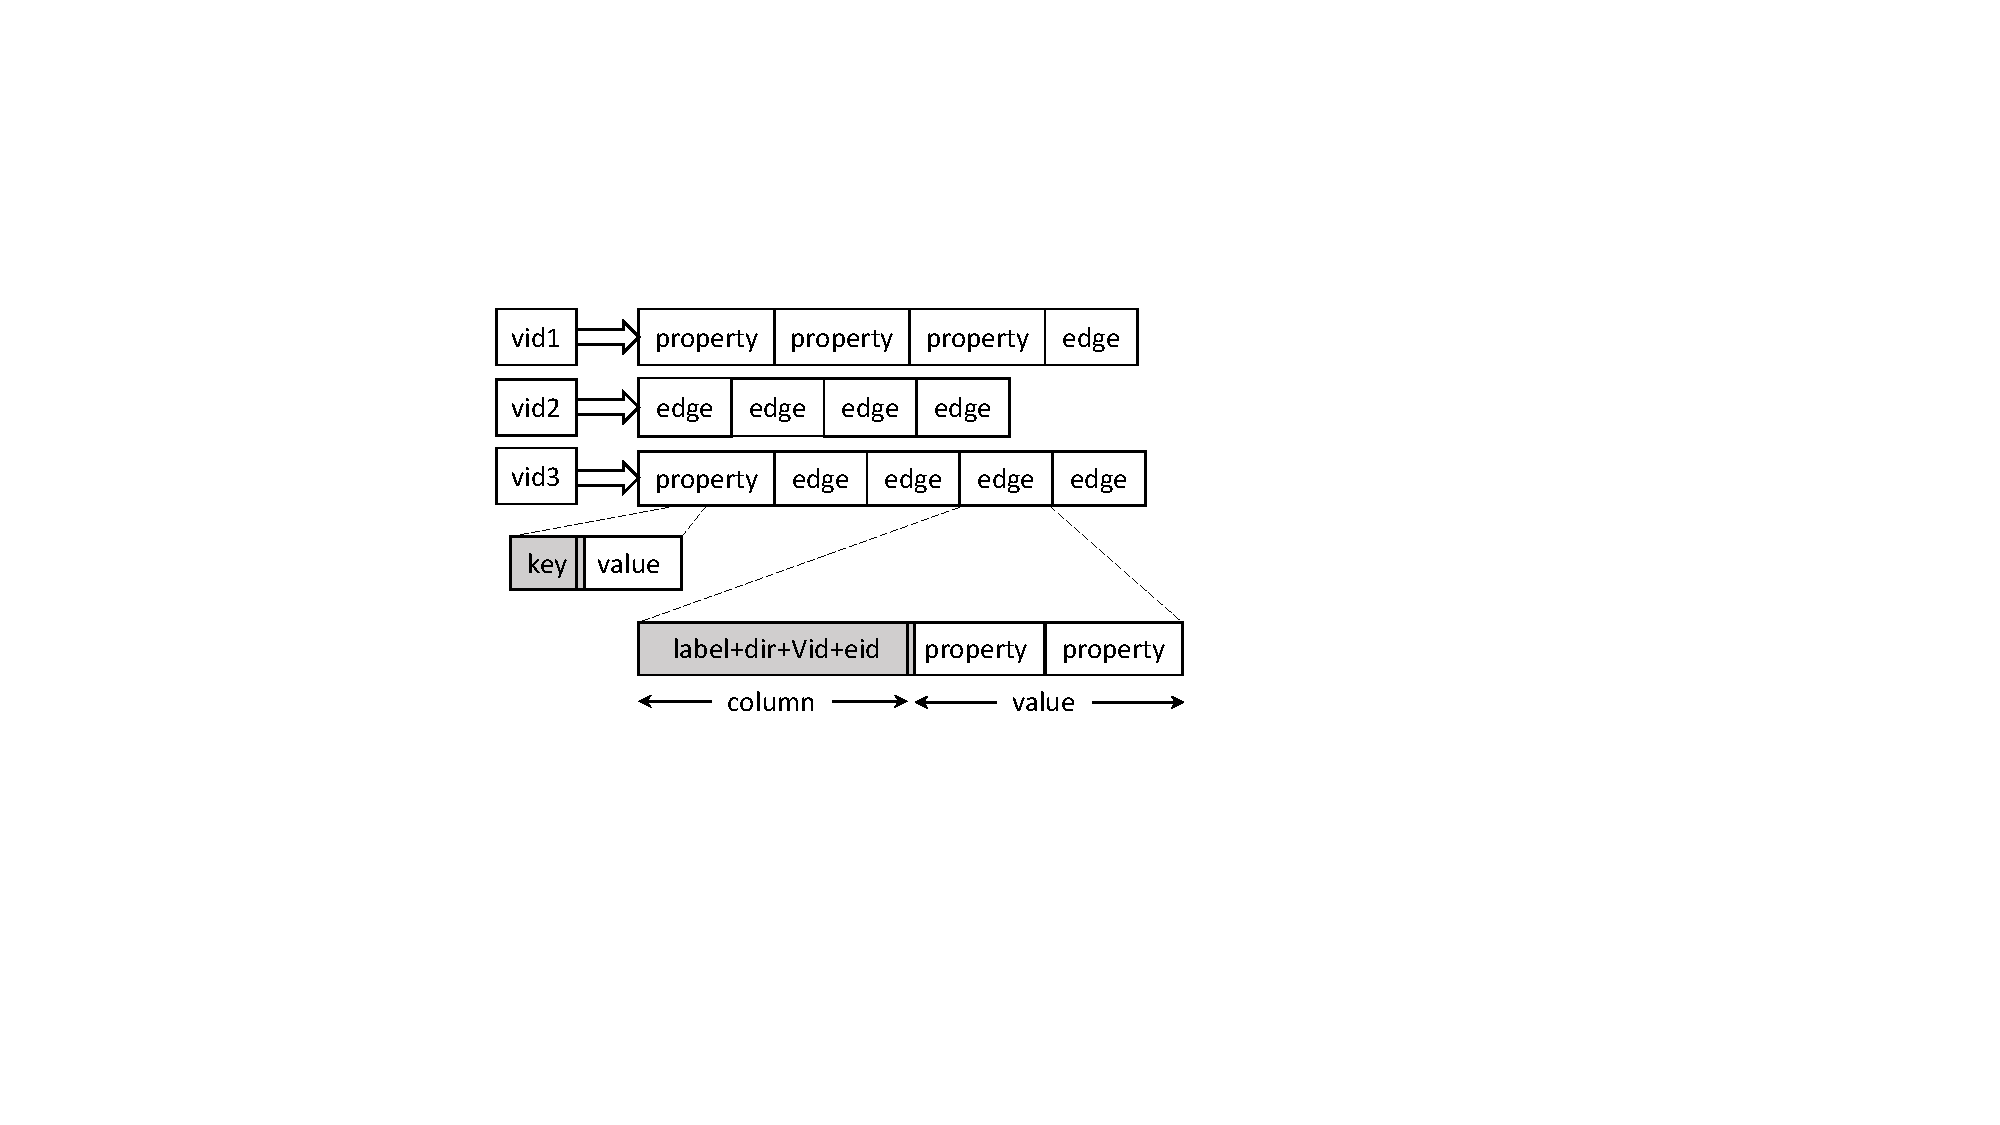
\includegraphics[width=100mm]{fig/adj_list.pdf}
\caption{Titan内部的BigTable实现}
\label{fig:adj_list}
\end{figure}

Titan为每个点分配了一个全局唯一的id,每个点占BigTable中的一行,行键就是点的id。每行存储了该点相关的属性和边,它们各占一个单元格。Titan在BigTable模型中设置最大版本数为1,从而使每行中的列名与单元格一一对应,根据行键和列名可以快速定位到目标单元格,实现对边和属性内容的快速检索。
在Titan中,每个属性是一个key-value对。点的属性存储在该点所在的行,每个属性占一个单元格,并以属性名key作为列名,这使得每个点的属性查询可以非常高效。
每个点所在的行还存储了邻接的所有边数据,每条边占一个单元格。一条边的信息包含了邻接点、类别(label)、方向、边的唯一id,以及边上的各属性。单元格的值用来存储边上的所有属性,列名则存储边上除属性外的其它信息。在BigTable模型中,同一行的单元格按列名排序。为了方便检索,每条边所在的单元格依次以label、方向、邻接点id以及边id拼接成为列名,即
\begin{center}
  列名 = 边label + 方向 + adjVid + eid
\end{center}
这种列名设计使得一个点的所有边先按label排序,再按方向、邻接点id、边id等排序。其优点是当要检索该点指定label的所有边时,只需要扫描邻接表的一部分。图4是一个更详细的示例。

\section{图数据库Titan的局限性}
当图中的重边数量巨大时,Titan的邻接表列数也急剧变大,这会对邻域中点和边的检索带来严重影响。

\begin{figure}[htbp]
\centering
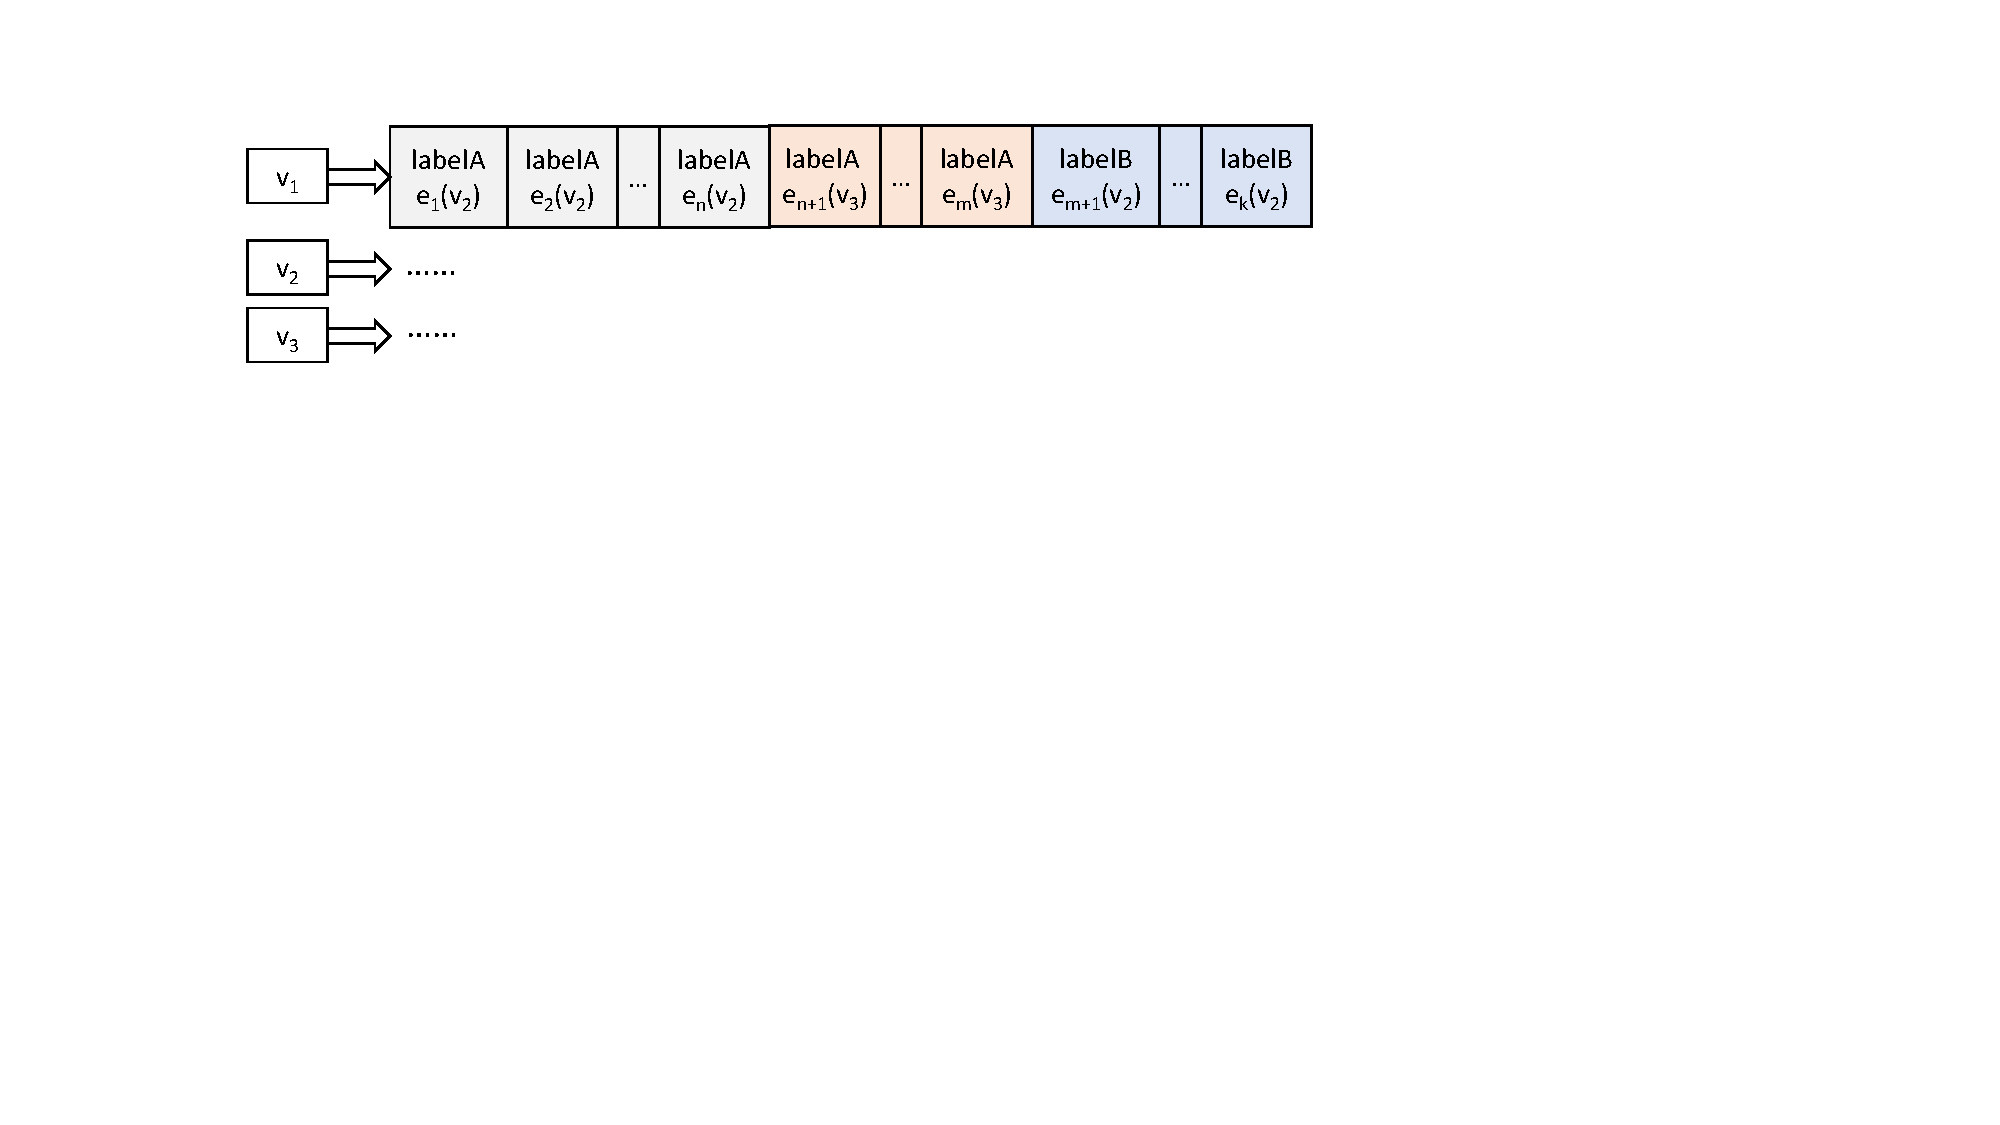
\includegraphics[width=150mm]{fig/original_list.pdf}
\caption{当属性图富含重边时,Titan在HBase中的数据表是一张扁平而宽的表}
\label{fig:orginal_list}
\end{figure}

图\ref{fig:orginal_list}展示了一个富含重边的场景,为方便展示省略了边的方向。v1只有v2和v3两个邻接点,其中与v2有两种label的边,与v3有一种label的边。虽然邻接的点数不多,但v1与邻接点都有数量巨大的重边。由于邻接表存储的是每条边的信息,当要查询v1的所有邻接点集(即v1、v2)时,不得不遍历一次v1的所有边,即遍历整个邻接表。当重边数量巨大时,这是大量的无谓开销。
为了规避上述情形,我们可以换一种列名设计来优化邻域点集查询,比如让邻接表先按邻接点id排序,令
\begin{center}
  列名 = adjVid + 边label + 方向 + eid
\end{center}
这样当发现一个邻接点时,可以跳过相同邻接点的所有边,不用再遍历整个邻接表。然而,面对label相关的查询时又会面临同样的问题,比如查询该点总共有几种label的边,仍需要遍历该点的整个邻接表。因此,改变邻接表的列名设计并不能解决问题,本质原因是邻接表存储了所有的边集。
另一方面,Titan为加快数据访问设计了缓存,存储最近访问的点及其邻接表内容。如果图中各点的重边都很多,则缓存空间被大量的重边占满。由于是重边,这些边中只有为数不多的邻接点。在做邻域点集相关查询时就会极大增加缓存的失效率。
面对富含重边的属性图,把所有边集都存在邻接表中是Titan性能受损的原因所在。


% vim:ts=4:sw=4
